\documentclass[a4paper, 11pt]{article}

\usepackage[english]{babel}
\usepackage[utf8]{inputenc}
\usepackage[T1]{fontenc}
\usepackage{graphicx}
\usepackage{color}
\usepackage{amsmath,amssymb}
\usepackage{rotating} 
\usepackage{layaureo}
\usepackage{booktabs}
\usepackage{varioref}
%\usepackage{subfigure}
\usepackage{listings}
\usepackage{wrapfig}
\usepackage{siunitx}
\usepackage{physics}
\usepackage{subcaption} 
\usepackage{subfloat}
\usepackage{caption}
\usepackage{gensymb}

\sisetup{output-decimal-marker={.}}

\author{Jakub Skowronski & Alessandro Compagnucci}
\title{Advanced Physics Laboratory Report:}

\begin{document}


\maketitle

\section{Introduction}
 \paragraph{}
 
We are using a silicon detector of $200$ $\mu$$m$ thickness, which completely stops the incoming low energy charged particles ($\alpha$ or $p$) inside it. These charged particles cannot come out of the detector and this will be an issue to plot $\Delta$E-E graph, which is used to identify the incoming charged particle. For the particles stopping in the thin silicon detectors, it is foreseen to employ pulse shape discrimination techniques to discriminate between them. It is thus critical to preserve the shape of the original signal, in particular considering that the distance between the reaction chamber and the readout electronic is approximately 10m. For this reason, a second stage of signal treatment was added in the electronic chain between the pre-amplifiers and the readout which transform the signal from single-ended to differential module. Instead if we use the single ended amplifier the signal gets integrated over the entire length of the cable and information regarding the shape of the signal is lost and hence we will not be able to exactly identify the incoming charged particle.
         
These voltage signals can be analyzed offline. These signals carry the information on energy of the incoming particle and type of incoming particle.  To understand the type of the incoming particle we need to do the pulse shape analysis i.e. the rise time, fall time will be different for different types of incoming particles. But the exact information on the energy of the incoming particle is given by the height of the signal.The peak of these signals carry the information about the charge collected from the detector which is proportional to the energy of the incoming particles.
 

\paragraph{}
In the  second section of this report , the setup used to investigate the linearity of the electronic chain with respect to the amplitude of the input signal is described. In the third section, the characterization of the detectors with an alpha source is presented.In the second and third section results are also discussed,which basically emphasizes that the setup we are using is linear with respect to the energy incident on the detector and linearity is retained throughout the setup. The excellent energy resolution obtained and the linearity of the setup make it usable for spectroscopic studies. Moreover, the possibility to identify charged particles and light nuclei using pulse shape discrimination (for low energy particles) and/or E-$\Delta$E methods makes the setup versatile and of great interest for gamma spectroscopy.This setup when used in coincidence with the gamma detector it can reveal more information on the reaction dynamics and the decay of the nuclei produced in the reaction.


\section{Linearity of the Electronic Chain}
Checking the linear response of the electronic chain is an important step in any of the nuclear physics experiment. If we basically look at the experimental apparatus we are using we realize that in order to get the exact information about the energy of the incident particle, the response of each and every electronic device which we are using should behave linearly with respect to the energy of the incident particle. So in order to verify the above statement we constructed the chain as shown below and checked it.

\begin{figure}[h]
    \centering
    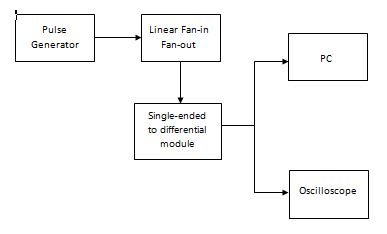
\includegraphics[scale = 0.5]{electronic_chain_diagram.JPG}
    \caption{Electronic chain}
    \label{fig:my_label}
\end{figure}


As in the above diagram pulse generator from the Berkeley nucleonics had to be connected to a linear Fan in Fan out module which basically reproduces the same pulse in 12 different ports. These 12 signals from Fan-in Fan-out circuit had to be connected to the Single-ended to differential module. In order to do so we made the cables for the 12 outputs from Fan-in Fan-out module by soldering and we connected it. The output of the differential amplifier is as shown in the following picture:


\begin{figure}[h]
 
\begin{subfigure}{0.5\textwidth}
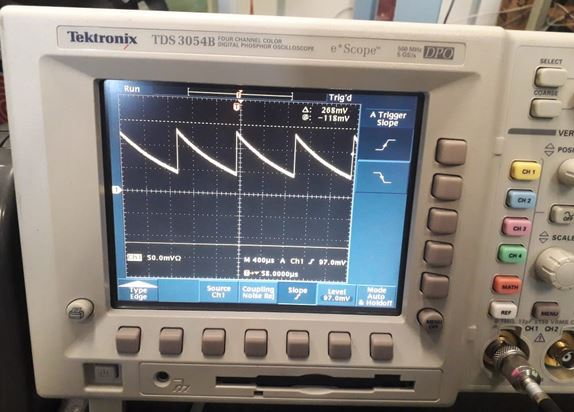
\includegraphics[width=0.9\linewidth, height=5cm]{test_signal_oscilloscope.JPG} 
\caption{output as seen in oscilloscope}
\label{fig:subim1}
\end{subfigure}
\begin{subfigure}{0.5\textwidth}
\includegraphics[width=0.9\linewidth, height=5cm]{test_signal_pc.JPG}
\caption{output as seen in pc}
\label{fig:subim2}
\end{subfigure}
 
\caption{Input pulse characteristics $a)$ $Wave-form$ $:$ $Square-wave$ \newline $b)$ $Amplitude$ $:$ $0.2V$ and $c)$ $Fall-time$ $:$ $1ms$}
\label{fig:image2}
\end{figure}


We know that the height of the signal gives us the information on the energy of the incident particle. So our next step was to measure the  height of the signal. As it can be seen that if the peak of the signal is present only for a small duration of time then it will be a very difficult task to determine the energy as Data Acquisition system should exactly take the reading at that instant of time or-else the energy information will be wrong. So what is generally done is the signals are treated with a trapezoidal filter with a characteristic rise time and a flat width. Now the advantage is that the information on the peak of the signal is available for the longer duration of time and it will not be a problem for the data acquisition and there by we get the exact information on the energy of the incident particles.
In this procedure of Parametrization of signal we should be careful of the frequency of the signals, because higher the frequency the probability of the overlap between the edge of the signal with the tail of the previous signal is more and this might create new set of problems in our analysis.  In this parametrization procedure we have 3 important parameters and they are $decay$ $constant$, $the$ $rise$ $time$ and $flat$ $top$ $width$.
\paragraph{}
Once the optimal parameters of the trapezoidal filter were found for a given amplitude, the linearity of the response function of the acquisition chain was tested. For this purpose, the amplitude of the input signal was varied between 0.2 and 1.6 V, as the maximum voltage acceptable for the  digitizer is 2 V peak-to-peak. The amplitude of the signal extracted from the trapezoidal filter for the different amplitudes is reported in Fig. 3. A linear fit was made and the results are reported on the figure. 


\begin{figure}[h]
    \centering
    \includegraphics[width=0.75\textwidth]{Graph1.jpg}
    \caption{Evolution of the measured amplitude of the signal with the trapezoidal filter in function of the set amplitude of the signal}
\end{figure}

The above graph is for one of the twelve channels.In the above graph along the y axis we have the amplitude of the input signal and in the x axis we have channel number of the peak of the histogram. From the above graph we get the trend line and the expected value for each and every point which is required for us to plot the residual graph which is  as shown below :
\begin{figure}[h]
    \centering
    \includegraphics[scale = 0.5]{calib_0_new.png}
    \caption{Residual plot for channel 0, where y axis is standard deviation in the gaussian fit of the histogram peak and the x axis is voltage }
    \label{fig:my_label}
\end{figure}



 Important thing to be noted from this graph is that the points in a residual plot are randomly dispersed around the horizontal axis,this tells us that the behaviour is linear i.e. this behaviour can be explained by the linear models.This tells us that the output from the electronic chain is linear with respect to the amplitude of the input signal and verifies the linearity of the electronic chain we are using in the data acquisition during an experiment.
We also performed the same analysis using the one more different single ended to differential module and found the similar behaviour. All the graphs have been added at the end of this report. In the next section we have combined this electronic chain with the silicon detector (TRACE) and performed the similar analysis. 


\section{TRACE Detector}
TRACE means TRacking Array for Charged Ejectiles.In order to connect the integrated charge-sensitive pre-amplifiers to the TRACE silicon detector prototypes a custom board was designed and realized.Each board can host 2 ASIC pre-amplificators designed by INFN Milano and University of Milano with 8 channels each. The ASICS can be reconfigured using different soldering in order to accept the back channel. As each detectors is segmented in 60 pads of 4 mm2, a total of 4 pre-amplification boards are required by telescope.
The amplified signals is going out of the chamber via a flat cable connected to a FISCHER 27-pins connectors feedthrough making the bridge between the reaction chamber under vacuum (10e-3 mbar) and the laboratory. Outside of the chamber, from each FISCHER connector, the cables are divided in two 12-pins MOLEX connectors mounted on the Single-ended-to-differential modules. From here we go directly to the 14-bits 100 MHz home made digitizer of the GALILEO array using MDR-26 connectors and 10 m cables.


\paragraph{}
The  output  signals  are  routed  to  three $MDR - 26$  connectors.Proper adapters were used to connect the board to the array of $3M$ headers on the flange of the vacuum chamber. They are FPGA-powered 100 MHz 14-bit resolution digitizer cards with four  differential  inputs  each.  A triple alpha source was put inside the vacuum chamber.  The  system  was  operated  at  $0.2$  $mbar$.  The  energy resolution at different energies is reported in the different channels is as shown below:
 
\begin{figure}[h]
 
\begin{subfigure}{0.5\textwidth}
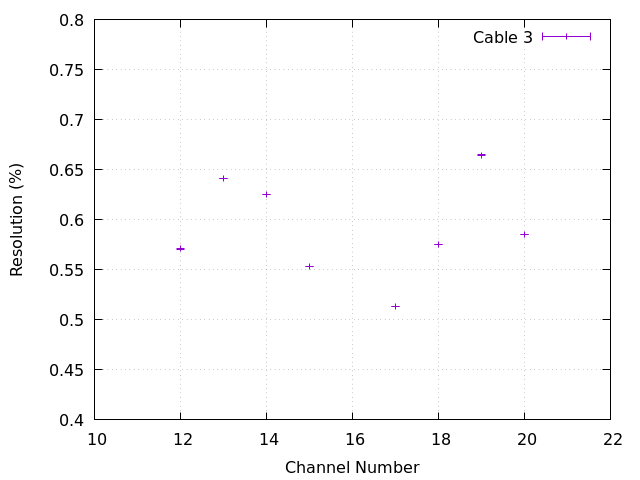
\includegraphics[width=0.9\linewidth, height=5cm]{3_res_am.png} 
\caption{Americium-241}
\label{fig:subim1}
\end{subfigure}
\begin{subfigure}{0.5\textwidth}
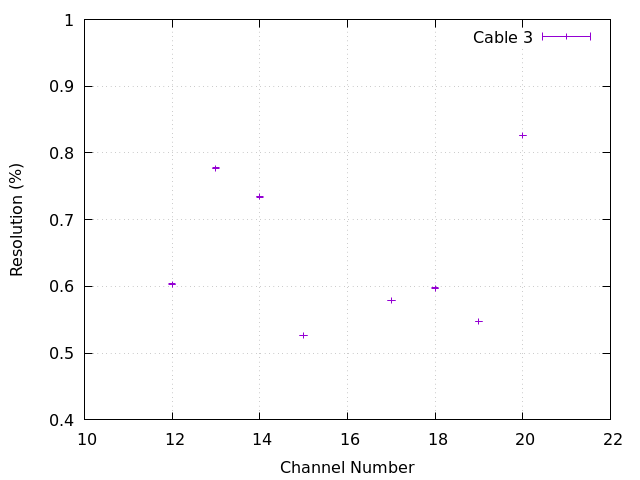
\includegraphics[width=0.9\linewidth, height=5cm]{3_res_cm.png}
\caption{Curium-244}
\label{fig:subim2}
\end{subfigure}

\begin{subfigure}{0.5\textwidth}
\centering
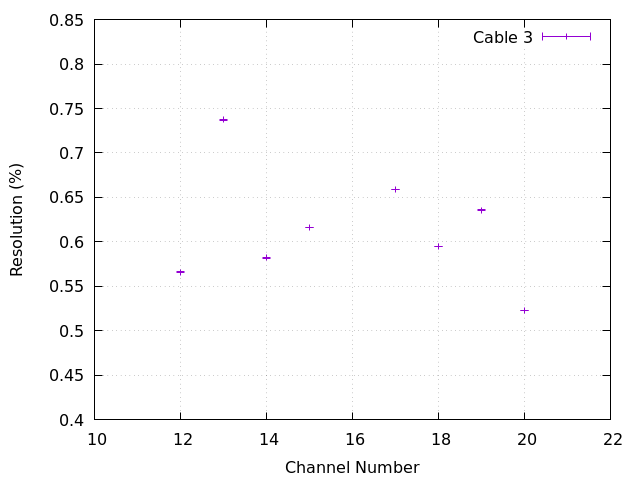
\includegraphics[width=0.9\linewidth, height=5cm]{3_res_pu.png}
\caption{Plutonium-239}
\label{fig:subim2}
\end{subfigure}

\caption{Resolution of various channels with triple $\alpha$ source}
\label{fig:image2}

\end{figure} 
The following table contains the most important $\alpha$  emissions from the triple $\alpha$  source.

\begin{center}
\begin{tabular}{ |c|c| } 
 \hline
 Source & $E$_$\alpha$ ($MeV$)  \\ 
 \hline
 239Pu & 5.1566  \\
 \hline
 241Am & 5.4856  \\ 
 \hline
 244Cm & 5.8048 \\
 \hline
\end{tabular}
\end{center}


 
Data acquisition is triggered through the channel $0$ (electron collection side). We are changing the channels in the detectors and using the triple alpha source we have checked for the resolution of all the different parts of the detector. The connection through different channels in the vacuum chamber gives the signal in one particular set of the channels. Each output channel in the vacuum chamber is connected to the $8$ panels in the tkt screen. We acquire data for some time and then apply trapezoidal filter to fit the the data peaks with a gaussian curve to get the exact location of the peak i.e. the centroid  and assign the value alpha source energy to that particular channel and thereby calibrate the entire detector for the energy of the incoming particle. The experimental setup is as shown below :


\begin{figure}[h]
 
\begin{subfigure}{0.5\textwidth}
\includegraphics[width=0.9\linewidth, height=5cm]{20190603_155227.jpg} 
\caption{source is placed very close above the detector}
\label{fig:subim1}
\end{subfigure}
\begin{subfigure}{0.5\textwidth}
\includegraphics[width=0.9\linewidth, height=5cm]{20190603_155221.jpg}
\caption{connections from the detector to the pre-amplifiers}
\label{fig:subim2}
\end{subfigure}
%\caption{experimental setup}
\label{fig:image2}



\begin{subfigure}{0.5\textwidth}
\includegraphics[width=0.9\linewidth, height=5cm]{expt_1.jpeg} 
\caption{experimental setup is placed in the vacuum chamber}
\label{fig:subim1}
\end{subfigure}

\caption{experimental setup}
\label{fig:image2}
\end{figure}

In conclusion, as part of this laboratory we have investigated the response function of a full acquisition chain. Starting from the detector, we started by producing the cables to go from the detector to the pre-amplification boards and the adapter for the pulser test-bench. The linearity of the newly designed and produced single-ended to differential modules has been tested using a high-precision PB-5 pulser, resulting in a very good linearity for the foreseen application of the detector. After this initial step, we characterized one detector and its acquisition chain in terms of energy resolution for different parameter of the signal treatment. This necessary work will be used for on-going experiment at the Legnaro National Laboratories for the study of clustering in light nuclei using direct reactions.  
 
      
      
\begin{figure}
 
\begin{subfigure}{0.5\textwidth}
\includegraphics[width=0.9\linewidth, height=5cm]{calib_0_new.png} 
\caption{channel 1}
\label{fig:subim1}
\end{subfigure}
\begin{subfigure}{0.5\textwidth}
\includegraphics[width=0.9\linewidth, height=5cm]{calib_1_new.png}
\caption{channel 2}
\label{fig:subim2}
\end{subfigure}

\begin{subfigure}{0.5\textwidth}
\includegraphics[width=0.9\linewidth, height=5cm]{calib_2_new.png} 
\caption{channel 3}
\label{fig:subim1}
\end{subfigure}
\begin{subfigure}{0.5\textwidth}
\includegraphics[width=0.9\linewidth, height=5cm]{calib_3_new.png}
\caption{channel 4}
\label{fig:subim2}
\end{subfigure}

\begin{subfigure}{0.5\textwidth}
\includegraphics[width=0.9\linewidth, height=5cm]{calib_4_new.png} 
\caption{channel 5}
\label{fig:subim1}
\end{subfigure}
\begin{subfigure}{0.5\textwidth}
\includegraphics[width=0.9\linewidth, height=5cm]{calib_5_new.png}
\caption{channel 6}
\label{fig:subim2}
\end{subfigure}

\begin{subfigure}{0.5\textwidth}
\includegraphics[width=0.9\linewidth, height=5cm]{calib_6_new.png} 
\caption{channel 7}
\label{fig:subim1}
\end{subfigure}
\begin{subfigure}{0.5\textwidth}
\includegraphics[width=0.9\linewidth, height=5cm]{calib_7_new.png}
\caption{channel 8}
\label{fig:subim2}
\end{subfigure}
\end{figure}

\begin{figure}[t]

\begin{subfigure}{0.5\textwidth}
\includegraphics[width=0.9\linewidth, height=5cm]{calib_8_new.png} 
\caption{channel 9}
\label{fig:subim1}
\end{subfigure}
\begin{subfigure}{0.5\textwidth}
\includegraphics[width=0.9\linewidth, height=5cm]{calib_9_new.png}
\caption{channel 10}
\label{fig:subim2}
\end{subfigure}

\begin{subfigure}{0.5\textwidth}
\includegraphics[width=0.9\linewidth, height=5cm]{calib_10_new.png} \caption{channel 11}
\label{fig:subim1}
\end{subfigure}
\begin{subfigure}{0.5\textwidth}
\includegraphics[width=0.9\linewidth, height=5cm]{calib_11_new.png}
\caption{channel 12}
\label{fig:subim2}
\end{subfigure}
 
\caption{residual graphs verifying the linearity of the electronic chain used in the experiment with differential amplifier:1}
\label{fig:image2}
\end{figure}


\begin{figure}
 
\begin{subfigure}{0.5\textwidth}
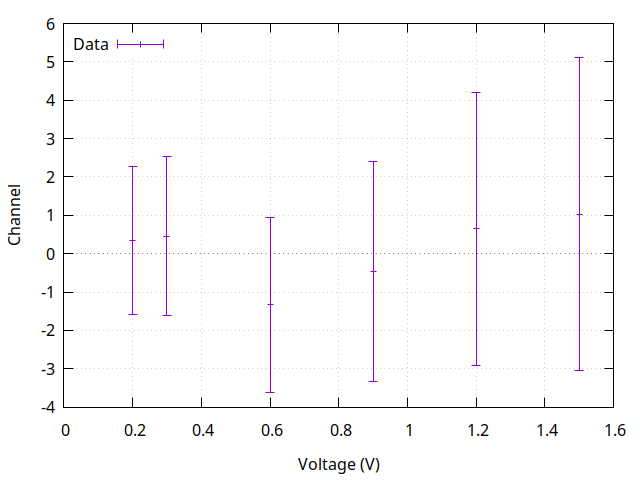
\includegraphics[width=0.9\linewidth, height=5cm]{calib_0.png} 
\caption{channel 1}
\label{fig:subim1}
\end{subfigure}
\begin{subfigure}{0.5\textwidth}
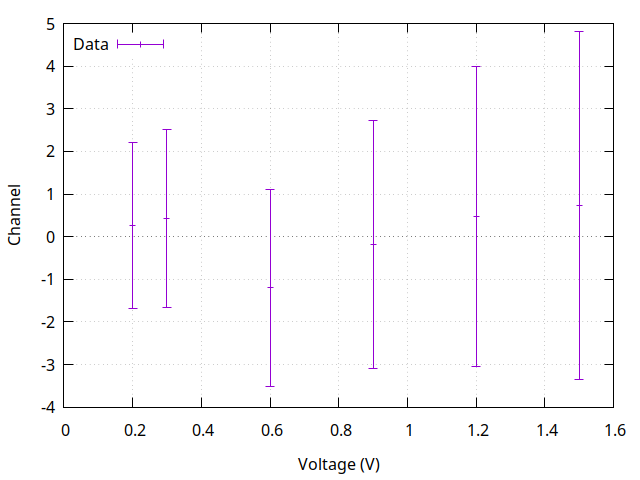
\includegraphics[width=0.9\linewidth, height=5cm]{calib_1.png}
\caption{channel 2}
\label{fig:subim2}
\end{subfigure}

\begin{subfigure}{0.5\textwidth}
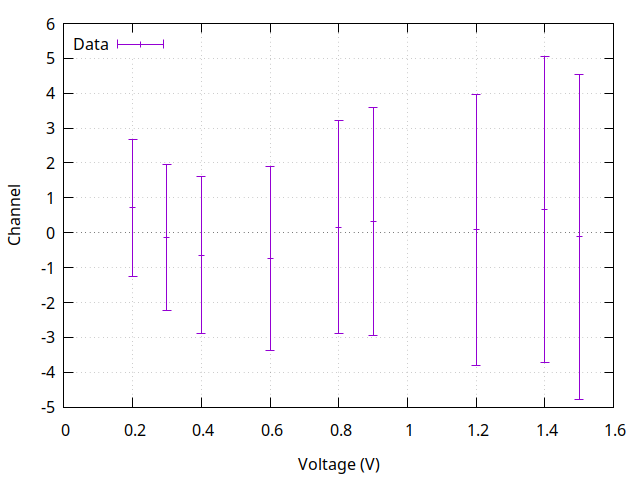
\includegraphics[width=0.9\linewidth, height=5cm]{calib_2.png} 
\caption{channel 3}
\label{fig:subim1}
\end{subfigure}
\begin{subfigure}{0.5\textwidth}
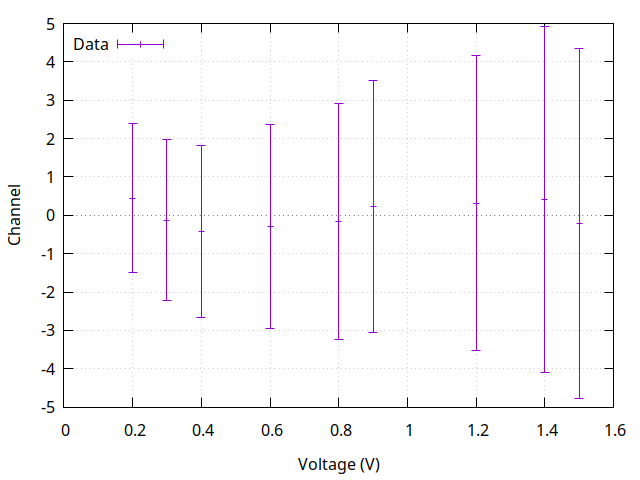
\includegraphics[width=0.9\linewidth, height=5cm]{calib_3.png}
\caption{channel 4}
\label{fig:subim2}
\end{subfigure}

\begin{subfigure}{0.5\textwidth}
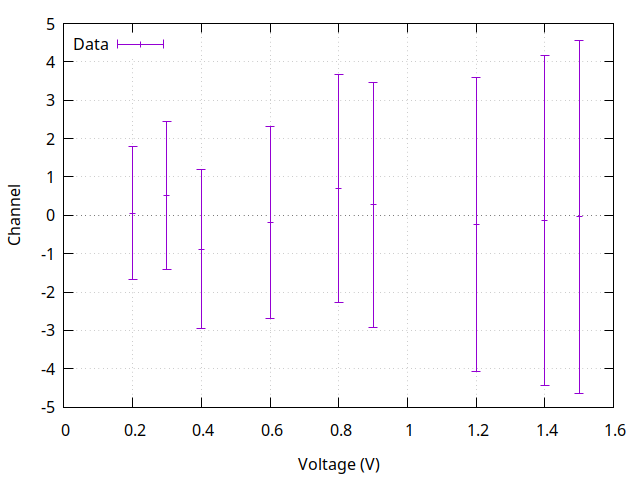
\includegraphics[width=0.9\linewidth, height=5cm]{calib_4.png} 
\caption{channel 5}
\label{fig:subim1}
\end{subfigure}
\begin{subfigure}{0.5\textwidth}
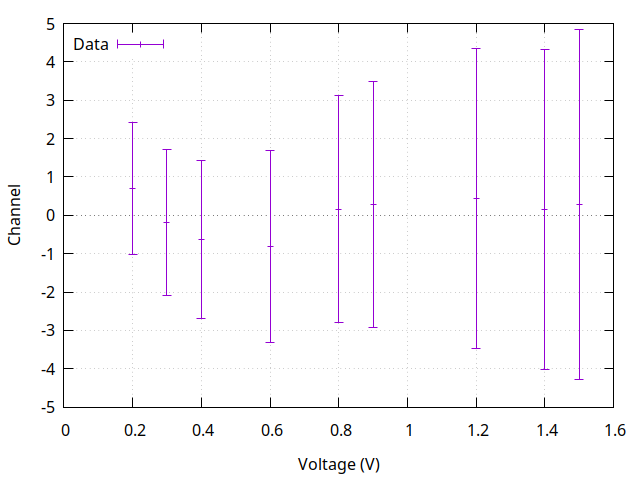
\includegraphics[width=0.9\linewidth, height=5cm]{calib_5.png}
\caption{channel 6}
\label{fig:subim2}
\end{subfigure}

\begin{subfigure}{0.5\textwidth}
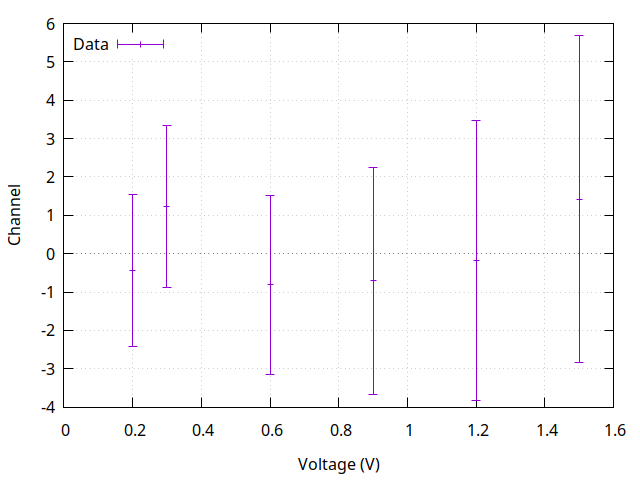
\includegraphics[width=0.9\linewidth, height=5cm]{calib_6.png} 
\caption{channel 7}
\label{fig:subim1}
\end{subfigure}
\begin{subfigure}{0.5\textwidth}
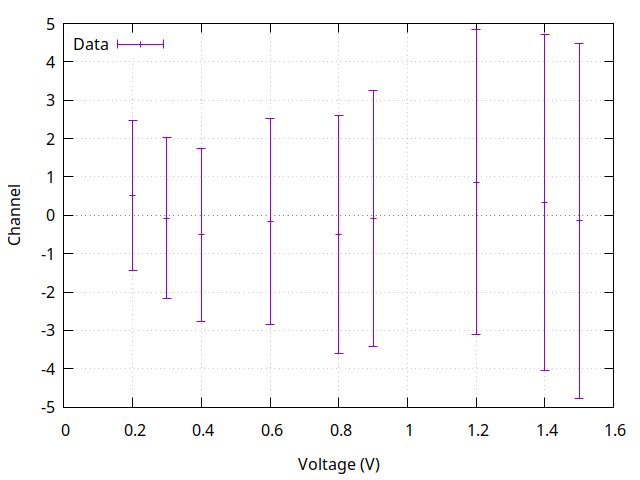
\includegraphics[width=0.9\linewidth, height=5cm]{calib_7.png}
\caption{channel 8}
\label{fig:subim2}
\end{subfigure}
\end{figure}

\begin{figure}[t]

\begin{subfigure}{0.5\textwidth}
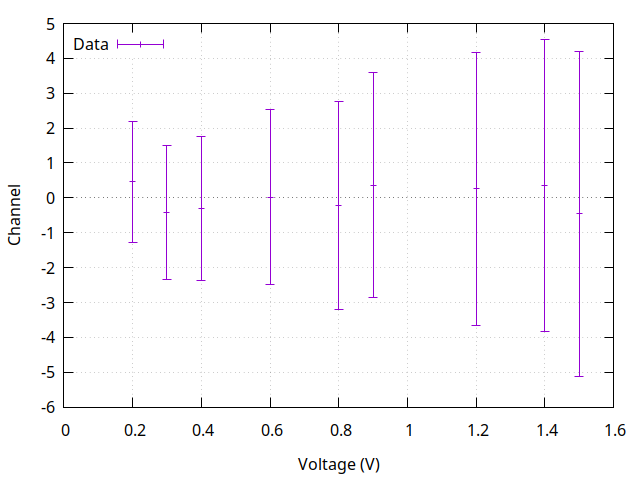
\includegraphics[width=0.9\linewidth, height=5cm]{calib_8.png} 
\caption{channel 9}
\label{fig:subim1}
\end{subfigure}
\begin{subfigure}{0.5\textwidth}
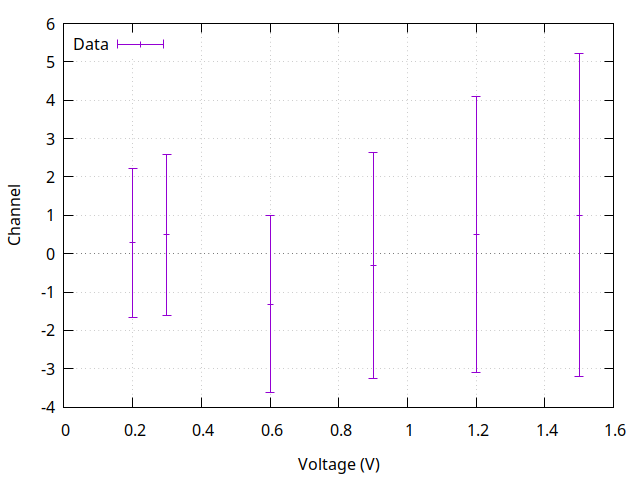
\includegraphics[width=0.9\linewidth, height=5cm]{calib_9.png}
\caption{channel 10}
\label{fig:subim2}
\end{subfigure}

\begin{subfigure}{0.5\textwidth}
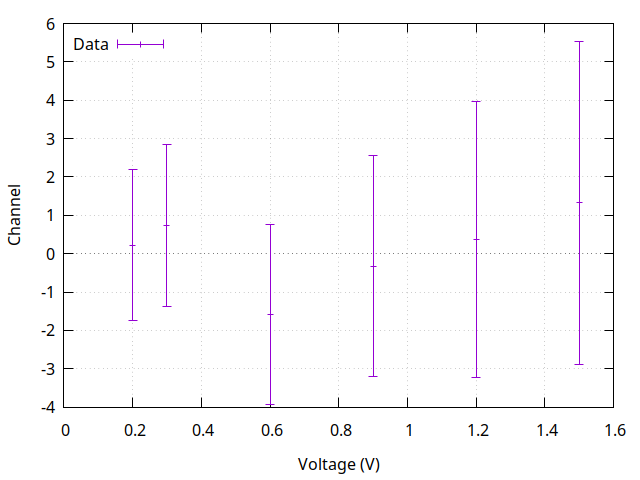
\includegraphics[width=0.9\linewidth, height=5cm]{calib_10.png} \caption{channel 11}
\label{fig:subim1}
\end{subfigure}
\begin{subfigure}{0.5\textwidth}
\includegraphics[width=0.9\linewidth, height=5cm]{calib_11_new.png}
\caption{channel 12}
\label{fig:subim2}
\end{subfigure}
 
\caption{residual graphs verifying the linearity of the electronic chain used in the experiment with differential amplifier:2}
\label{fig:image2}
\end{figure}

         
         
         
         
         
         
         
         
\end{document}
